\chapter{Solving Games Efficiently}

We have a formalism for the driver synthesis problem as a game. A practical driver synthesis tool using the game formalism must be able to solve and find strategies for these games for real device and operating system specifications in a reasonable amount of time. The principle challenge of this work is creating a synthesis algorithm that scales well enough to handle the large state machines of real device and operating system specifications. 

The straightforward symbolic solver that uses BDDs as the symbolic data structure is remarkably efficient. In fact, it is the current state of the art in reactive synthesis. I will use this as the starting point for my description of Termite's game solver.

I begin by describing my entry to the reactive synthesis competition in 2014, appropriately named "Simple BDD Solver". The solver won the sequential realizability category, the only category in which it was entered.  

Next, I introduce abstraction, a technique to increase the scalability of the basic symbolic algorithm by reducing the effective size of the state space that the algorithm must operate on. The cost of reducing the size of the state space is that the abstracted game is represented with less precision and is often not precise enough to solve the original game. To counter this, the abstraction needs to be \emph{refined}, i.e. the precision of the abstraction needs to be increased. This is performed in an \emph{abstraction-refinement loop}. Ideally, this loop results in an abstraction just precise enough to solve the game, but coarse enough that solving it is tractable.

I give an abstraction-refinement algorithm that uses \emph{variable abstraction}, a technique for reducing the state space of the game by eliminating a subset of the state variables from the game. I then build on this to arrive at an algorithm that performs \emph{predicate abstraction}, a technique that, instead of representing the state space using state variables, represents relationships between state variables that capture key properties that are likely to be of importance in solving the game. This representation is usually far more compact. This is the synthesis algorithm that Termite uses.

\section{Synthesis Competition}

The Reactive Synthesis Competition is a competition for reactive synthesis tools inspired by competitions in other fields such as the SAT competition and the Hardware Model Checking Competition. The competition had four tracks:
\begin{itemize}
    \item Sequential realizability
    \item Parallel realizability
    \item Sequential synthesis
    \item Parallel synthesis
\end{itemize}

The tools were required to solve safety games given in an extension of the AIGER format \cite{aiger}. 

Entrants in the synthesis categories were required to produce an implementation of a controller that enforced the safety condition, also given in extended AIGER format. Entrants in the realizability category were only required to determine if the safety game was winnable.

The Synthesis Competition was run as a satellite event to the CAV conference and Kurt Godel medals in silver were awarded to the winners of each category.

In the following sections I will describe my tool "Simple BDD Solver" which won the sequential realizability track.

\section{Symbolic Solver}
\label{sec:syntcomp}

The starting point for the design of an efficient game solver is the standard BDD-based symbolic algorithm of Section~\ref{sec:back_symbolic_alg}. This standard symbolic algorithm forms the basis of my entry to the Reactive Synthesis competition, named `Simple BDD Solver'. The basic algorithm admits a number of optimisations. As I will show in Section~\ref{sec:syntcomp_eval}, these optimisations significantly improve the performance of the algorithm, but not enough to synthesize even simple device drivers. Yet, this optimised symbolic algorithm is used inside the abstraction-refinement loop of Termite to solve the abstract games produced at every refinement iteration. I therefore describe each of them below.

This section focuses on safety games, as required for the synthesis competition. However, all of the optimisations presented here apply equally to reachability games and to the GR(1) games used in Termite. 

\subsection{Overview}
Following Section~\ref{sec:back_symbolic_alg}, the standard BDD-based symbolic algorithm computes:

\begin{equation}
\label{eqn:mu_syntcomp}
\nu X. Cpre(X \lor \sigma)
\end{equation}

\noindent where $\sigma$ is the safety condition.

The controllable predecessor (Section~\ref{sec:back_cpre}) is specific to the type of game being solved. I give the controllable predecessor for the synthesis competition below as it is simpler than Termite's and is used in the discussion of optimisations below.

\begin{equation}
\label{eqn:cpre_syntcomp}
Cpre(X) = \forall U. \exists C. \forall S'. (\delta(S, U, C, S') \rightarrow X')
\end{equation}

\noindent where $U$ is the set of valuations of uncontrollable inputs, $C$ is the set of valuations of controllable inputs, and $S$ is the set of valuations of state variables. Given a set $X$, $X'$ denotes the next state copy of $X$ and $\delta$ is the transition relation.

\subsection{Optimisations}
\label{sec:syntcomp_optimisations}

The optimisations that I have used, in approximate order of importance, are:
\begin{itemize}
    \item Dynamic variable reordering using the sifting algorithm \cite{Rudell_1993}
    \item Dereference unused BDDs as soon as possible
    \item Partitioned transition relations \cite{Burch_91} and direct substitution with \textsc{Cudd\_VectorCompose}
    \item Simultaneous conjunction and quantification with \textsc{Cudd\_BddAndAbstract}
    \item Terminate early where possible
\end{itemize}

The optimised algorithm (Algorithm~\ref{alg:syntcomp}) and controllable predecessor (Algorithm~\ref{alg:syntcomp_cpre}) are given in the implementation section (Section~\ref{sec:syntcomp_impl}).

\subsubsection{Dynamic variable ordering}
I do not try to find a good static variable ordering at the start and instead rely on the sifting algorithm provided by the CUDD package for finding good variable orderings dynamically. In my experience, the sifting algorithm provides the best tradeoff between the quality of the resulting ordering and time taken to find it. I enable sifting at the start so that it is active during both compilation and solving. I did not modify any of the default parameters to the sifting algorithm.

\subsubsection{Dereferencing dead BDDs}
I dereference BDDs that are no longer needed as soon as possible. Each live BDD node is processed during reordering and counted when the algorithm checks to see if the total BDD size in the manager is reduced. These unused BDDs should not count toward the total node count that is used to evaluate an ordering, and, the time that is spent reordering them is wasted. Furthermore, these unused BDDs occupy memory and, if not dereferenced, may use up all of the memory available on the system.

\subsubsection{Partitioned transition relations}
\label{sec:syntcomp_partitioned}
I do not compute the transition relation as a monolithic BDD defined over current state, input variables and next state. This would likely be very large and slow down the algorithm considerably. Instead, I keep it in a conjunctively partitioned form with one partition for each next state variable as described below. 

This optimisation is sound because the next state value of any state variable depends only on the current and input variables and not any other next state variables. Furthermore, the next state value of any state variable is deterministic. This means that it can be represented directly as a function of the current state and input variables. I use a BDD defined over current state and input variables to represent this function. The transition relation becomes a list of BDDs, one for each state variable, each of which only depends on current state and input variables. 

To compute the implication, $\forall S'. (\delta(S, U, C, S') \rightarrow X')$, I use the CUDD function \textsc{Cudd\_VectorCompose} as shown in algorithm \ref{alg:syntcomp_cpre} on line~\ref{l:vc} to substitute each update function into X. This avoids building the monolithic transition relation and, importantly, it avoids having to ever declare a next state copy of each state variable in the BDD manager. 

\subsubsection{Simultaneous conjunction and quantification}
I perform simultaneous conjunction and existential quantification wherever possible. CUDD implements a composite operation that performs quantification and conjunction simultaneously called \textsc{Cudd\_BddAndAbstract}. Given two BDDs $x$ and $y$ and a set of variables $v$, it computes $\exists v. x \land y$ as a single operation without explicitly building the conjunction $x \land y$. I perform this optimisation on line~\ref{l:andabs} of Algorithm~\ref{alg:syntcomp_cpre}. As this avoids building the potentially large BDD representing the conjunction it saves both memory and time.

\subsubsection{Early termination}
I terminate early when possible. As I am computing a greatest fixed point, I start with the universal set and progressively shrink it to find the winning region. Each time I shrink the winning region, I check that is it still a superset of the initial set. If it is not, I know there is no way player~1 can win as the winning set only shrinks as the algorithm progresses. I use the function \textsc{Cudd\_bddLeq} on line~\ref{l:leq} of Algorithm~\ref{alg:syntcomp} for this purpose as it efficiently checks that one BDD implies another without constructing the BDD of the implication.

\subsection{Implementation}
\label{sec:syntcomp_impl}
I developed two implementations that incorporate all of the above optimisations. The first implementation is used by Termite inside the abstraction refinement loop in order to solve abstract games (Section~\ref{sec:abs_ref_pred_abs}). The second solver was developed for the reactive synthesis competition. 

The Reactive Synthesis Competition~\cite{syntcomp_arxiv} is a competition for reactive synthesis tools inspired by competitions in other fields such as the SAT competition~\cite{satcomp} and the Hardware Model Checking Competition~\cite{hwmcc}. The competition had four tracks: sequential realisability, parallel realisability, sequential synthesis and parallel synthesis. The tools were required to solve safety games given in an extension of the AIGER format \cite{aiger}. Entrants in the synthesis categories were required to produce an implementation of a controller that enforced the safety condition, also given in extended AIGER format. Entrants in the realisability category were only required to determine if the safety game was winnable, not to produce a strategy.

Two different implementations were required because the synthesis competition requires a different controllable predecessor to driver synthesis (Section~\ref{sec:termite_cpre}), and, modifications to allow for predicate abstraction were necessary for Termite (Section~\ref{sec:abs_ref_pred_abs}).

The synthesis competition solver is written in the Haskell functional programming language. It uses the CUDD \cite{cudd} package for binary decision diagram manipulation and the Attoparsec Haskell package for fast parsing. Altogether, the solver, AIGER parser, compiler and command line argument parser are just over 300 lines of code. The code is available online at: \path{https://github.com/adamwalker/syntcomp}.

\begin{algorithm}
\caption{Syntcomp Controllable predecessor}
\label{alg:syntcomp_cpre}

\begin{algorithmic}[1]

\Function{CPre}{$C, U, \sigma, target$}

\State $substituted \gets \Call{Cudd\_VectorCompose}{target, \delta}$ \label{l:vc}
    \State $safeSub     \gets \Call{Cudd\_bddAndAbstract}{C, \sigma, substituted}$ \label{l:andabs}
    \State $winning     \gets \Call{Cudd\_bddUnivAbstract}{U, safeSub}$
    \State \Return $winning$

\EndFunction

\end{algorithmic}
\end{algorithm}

\begin{algorithm}
\caption{Syntcomp symbolic solver}
\label{alg:syntcomp}

\begin{algorithmic}[1]

\Function{Solve}{$\sigma, init, \delta, C, U$}

    \State $win \gets \Call{Cudd\_ReadLogicOne}{}$
    \Loop
        \State $res' \gets \Call{CPre}{C, U, \sigma, res \land \sigma}$
        \State $win  \gets \Call{Cudd\_bddLeq}{init, res'}$ \label{l:leq}
        \If{$\neg win$} 
            \State \Return $False$
        \EndIf
        \If{$res = res'$} 
            \State \Return $True$
        \EndIf
        \State $res \gets res'$
    \EndLoop

\EndFunction

\end{algorithmic}
\end{algorithm}

The optimised algorithm is given in Algorithm~\ref{alg:syntcomp}. It calls the optimised controllable predecessor suitable for the synthesis competition defined in Algorithm~\ref{alg:syntcomp_cpre}.

\subsection{Evaluation of Optimisations}
\label{sec:syntcomp_eval}

\begin{sidewaystable}
    \small
    \center
    \begin{tabular}{|l|S[table-format=2.2]|S[table-format=2.2]|S[table-format=2.2]|S[table-format=2.2]|S[table-format=2.2]|S[table-format=2.2]|}
        \hline
        \multirow{2}{*}{Benchmark} & \multicolumn{6}{c|}{Optimisation} \\ \cline{2-7} & 
        \multicolumn{1}{c|}{None}   & \multicolumn{1}{c|}{+ Reord.} & \multicolumn{1}{c|}{+ Deref.} & \multicolumn{1}{c|}{+ Partitioned} & \multicolumn{1}{c|}{+ Simult. abs.} & \multicolumn{1}{c|}{+ Early term.} \\
        \hline

        amba02\_new\_08n\_unreal.aag    & 34.73  & 37.00    & 1.15     & 0.63          & 0.28           & 0.22          \\
        amba02\_new\_08n\_unreal\_o.aag & 34.25  & 36.99    & 0.57     & 0.69          & 0.26           & 0.26          \\
        amba02\_new\_09n.aag            & 28.50  & 28.37    & 0.47     & 0.37          & 0.20           & 0.24          \\
        amba02\_new\_09n\_o.aag         & 28.20  & 30.73    & 0.62     & 0.40          & 0.24           & 0.28          \\
        amba03\_new\_08n\_unreal.aag    & OOM    & 391.59   & 1.94     & 0.88          & 0.94           & 0.95          \\
        amba03\_new\_08n\_unreal\_o.aag & OOM    & 426.67   & 1.76     & 1.45          & 0.82           & 0.47          \\
        amba03\_new\_09n.aag            & OOM    & 452.90   & 3.98     & 1.78          & 0.89           & 1.13          \\
        amba03\_new\_09n\_o.aag         & OOM    & 453.70   & 5.51     & 2.05          & 1.13           & 1.13          \\
        amba04\_new\_24n\_unreal.aag    & OOM    & OOM      & 28.40    & 5.48          & 4.91           & 2.54          \\
        amba04\_new\_24n\_unreal\_o.aag & OOM    & OOM      & 11.11    & 15.73         & 3.33           & 4.65          \\
        amba04\_new\_25n.aag            & OOM    & OOM      & 11.60    & 7.89          & 4.25           & 4.48          \\
        amba04\_new\_25n\_o.aag         & OOM    & OOM      & 9.12     & 7.50          & 5.41           & 7.31          \\
        amba05\_new\_16n\_unreal.aag    & OOM    & OOM      & 11.86    & 12.93         & 6.97           & 5.13          \\
        amba05\_new\_16n\_unreal\_o.aag & OOM    & OOM      & 17.93    & 11.79         & 6.28           & 5.56          \\
        amba05\_new\_17n.aag            & OOM    & OOM      & 31.36    & 5.47          & 7.37           & 6.53          \\
        amba05\_new\_17n\_o.aag         & OOM    & OOM      & 15.90    & 10.61         & 5.00           & 3.87          \\
        amba06\_new\_20n\_unreal.aag    & OOM    & OOM      & 50.89    & 32.04         & 6.15           & 5.44          \\
        amba06\_new\_20n\_unreal\_o.aag & OOM    & OOM      & 55.96    & 31.94         & 11.04          & 7.08          \\
        amba06\_new\_21n.aag            & OOM    & OOM      & 49.15    & 27.95         & 11.07          & 11.98         \\
        amba06\_new\_21n\_o.aag         & OOM    & OOM      & 21.12    & 21.85         & 12.61          & 27.48         \\
        amba07\_new\_24n\_unreal.aag    & OOM    & OOM      & 67.95    & 21.37         & 19.68          & 17.76         \\
        amba07\_new\_24n\_unreal\_o.aag & OOM    & OOM      & 45.36    & 91.67         & 20.14          & 17.94         \\
        amba07\_new\_25n.aag            & OOM    & OOM      & 127.04   & 53.93         & 15.90          & 18.38         \\
        amba07\_new\_25n\_o.aag         & OOM    & OOM      & 51.00    & 51.10         & 24.50          & 18.33         \\

        \hline
    \end{tabular}
    \caption{Runtimes (in seconds) of the symbolic solver with the optimisation of Section~\ref{sec:syntcomp_optimisations} progressively enabled}
    \label{tab:syntcomp_optimisations}
\end{sidewaystable}

Table~\ref{tab:syntcomp_optimisations} gives the runtimes, in seconds, of the symbolic solver on a selection of benchmarks from the 2014 synthesis competition. Benchmarks from the AMBA category were used. These benchmarks model an arbiter for the AMBA AHB bus, based on an industrial specification by ARM. The benchmarks were run on an Intel Haswell laptop with 4 gigabytes of ram and a processor speed of 1.6 GHz. Benchmarks containing the text `unreal' in the name are unsatisfiable and all others are satisfiable. If the runtime is listed as OOM, it means that the solver ran out of memory.

The first column gives the runtimes for the symbolic solver without optimisations. Most entries are failures due to out of memory conditions. I have enabled the optimisations progressively in subsequent columns. In the next two columns, dynamic variable reordering and BDD dereferencing are enabled. It is clear that these optimisations are crucial to the performance of the algorithm. In subsequent columns, I enable partitioned transition relations and simultaneous conjunction and quantification. These optimisations successively improve performance on nearly all benchmarks. Finally, in the last column, I enable early termination. This does not improve performance on many of the benchmarks. Early termination can only help when the benchmark is unsatisfiable. When the benchmark is satisfiable it only imposes the additional work of checking containment in the initial set. This optimisation does, however, improve performance substantially on some of the unsatisfiable benchmarks. It is unclear whether it is worthwhile.

The benchmark runner is available online at: \url{https://github.com/adamwalker/syntcomp-benchmark}. The set of benchmarks is available online at \url{https://syntcompdb.iaik.tugraz.at/static/SyntComp.tar.gz}.

\subsection{Conclusion}
Simple BDD Solver performed well compared to the other solvers entered in the reactive synthesis competition as a result of the optimisations presented above. It failed when the BDDs representing the winning sets, or the intermediate BDDs in the controllable predecessor computation grew too large. Additionally, it failed when a large number of iterations was required to determine the outcome, such as the benchmarks with a large counter. 



\section{Three Valued Abstraction-Refinement}
An abstraction is a simplification of the original transition system. An abstraction is used when the game is too large to be solved. Ideally, an abstraction is both small enough to be solved and detailed enough to gain some additional information about the properties of the system. 

One common use of an abstraction is in an abstraction-refinement loop. In an abstraction refinement loop, an initial simple abstraction is found and is solved. Then, the results of the abstraction are used to refine the abstraction, ie. to build another system model that contains slightly more detail than the original abstraction. This is repeated in a loop until the original game is solved. It is often possible to solve the original game with a far less detailed abstraction that the original system. 

Finding an abstraction that is simultaneously small and useful for making progress in solving the game is a difficult task and is what will be dealt with in the following sections. We start with earlier work on three valued abstraction refinement. 

\subsection{Three valued abstraction refinement}
\label{sec:three_val_abs_ref}

The idea is that given an abstraction, we classify states into one of three categories: winning, losing, and unknown. If we discover that the entire initial set is winning, we know that the original game is winning and we can terminate. Dually, if we discover any initial state that is losing, we know that the entire initial set can never be winning, hence the game is losing and we can terminate. 

At termination, either 
\begin{itemize}
\item all of the initial states are classified as winning (but the other states need not be classified), or
\item one of the initial states is classified as losing (again, no other states need to be classified)
\end{itemize}

This additional imprecision often allows us to use a less precise abstraction compared to the original algorithm where all states are exactly classified. The use of a coarser abstraction is usually computationally more efficient. If none of the termination conditions are met then we need to refine the abstraction. A correct abstraction refinement scheme will guarantee that one of the termination conditions is eventually met after enough refinements are performed. A good abstraction refinement scheme will ensure that when the algorithm terminates the abstraction is not unnecessarily fine.

\subsection{Abstraction}
\label{sec:abstraction_def}

An abstraction of a game structure $G$ is a tuple $\langle V, \concrete{}\rangle$, where 
\begin{itemize}
    \item $V$ is a finite set of abstract states and 
    \item $\concrete{} : V \rightarrow 2^S $ is the \emph{concretisation function}, which takes an abstract state and returns the possibly empty set of concrete states that the abstract state corresponds to.  
\end{itemize}
        
We require that 
\begin{itemize}
    \item $\bigcup_{v\in V}\concrete{v} = S$, ie. the abstraction covers the entire state space. 
    \item $\concrete{v_1}\cap \concrete{v_2} = \emptyset$ for any $v_1$ and $v_2$, $v_1 \neq v_2$, ie. the abstraction partitions the state space.
\end{itemize}

In the case when $\concrete{v} = \emptyset$ the abstract state $v$ is said to be \emph{inconsistent}. We extend the $\concrete{}$ operator to sets of abstract states as follows: for $U\subseteq V$: $\concrete{U} = \bigcup_{u\in U}\concrete{u}$.

\subsection{Algorithm}
\label{sec:threeval_generic}

In this section we present a modified version of the three-valued abstraction refinement technique of de~Alfaro and Roy~\cite{Alfaro_Roy_07}. To simplify the presentation, we focus on solving reachability games. 

We start by defining two versions of the abstraction operator: the \emph{may-abstraction} $\abstractm{}$ and the \emph{must-abstraction} $\abstractM{}$. For a set of concrete states $T \subseteq S$:

\begin{equation}
\abstractm{T} = \{v\in V\mid \concrete{v} \cap T \neq \emptyset\} 
\end{equation}

Intuitively, this returns the set of abstract states which, when concretised, overlap some element of the set to be abstracted.

\begin{equation}
\abstractM{T} = \{v\in V\mid \concrete{v} \subseteq T \}
\end{equation}

Intuitively, this returns the set of abstract states which, when concretised, are contained within the set to be abstracted.

We say that an abstraction is \emph{precise} for a set $T\subseteq S$ if :

\begin{equation}
\concrete{(\abstractm{T})} = \concrete{(\abstractM{T})}
\end{equation}

Intuitively, this means that there are no abstract states that, when concretised, contain states that within $T$ and states that are outside $T$.

Next, we define may and must versions of the abstract controllable predecessor operator:

\begin{equation}
    Cpre_i^m(U) = \abstractm{Cpre_i(\concrete{U})}
    \label{eqn:def_cpre_m}
\end{equation}

Intuitively, this returns the set of abstract states such that, when concretised, we can force execution from at least one concrete state into the concretisation of $U$.

\begin{equation}
    Cpre_i^M(U) = \abstractM{Cpre_i(\concrete{U})}
    \label{eqn:def_cpre_M}
\end{equation}

Intuitively, this returns the set of abstract states such that, when concretised, we can force execution from all of the concrete states into the concretisation of $U$.

These operators have the property:

\begin{equation}
\concrete{Cpre_i^M(U)} \subseteq Cpre_i(\concrete{U}) \subseteq \concrete{Cpre_i^m(U)}
\end{equation}

And therefore:

\begin{equation}
\label{eqn:cpre_inclusion}
\concrete{\reach(\abstractM{T}, Cpre_i^M)} \subseteq \reach(T, Cpre_i) \subseteq \concrete{\reach(\abstractm{T}, Cpre_i^m)}
\end{equation}

We denote $\reach(\abstractM{T}, Cpre_i^M)$ as $W^M$ and refer to it as the \emph{must-winning} region and we denote $\reach(\abstractm{T}, Cpre_i^m)$ as $W^m$ and refer to it as the \emph{may-winning} region.

\begin{figure}[t]
\centering
\includegraphics[width=0.85\linewidth]{diagrams/threeValOverview.pdf}
\caption{Overview of three valued abstraction-refinement}
\label{fig:three_val_overview}
\end{figure}

Figure~\ref{fig:three_val_overview} illustrates the main idea of three valued abstraction refinement, which is presented in algorithm~\ref{alg:generic}. The winning region, in grey, is overapproximated by the may-winning set in white and underapproximated by the must-winning set in dark grey. The abstraction-refinement loop progressively brings $W^m$ and $W^M$ closer together until the game outcome can be determined.

At every iteration, the algorithm computes the must-winning set $W^M$ that underapproximates, and the may-winning set $W^m$ that overapproximates the true winning set (lines~2--3).  The algorithm terminates if the must-winning set contains the entire initial set or the may-winning set has shrunk beyond the initial set (lines~4--5).  Otherwise, the algorithm attempts to refine the abstraction in a way that the must-winning set will be expanded in the next iteration when the game is re-solved.

\begin{algorithm}
\caption{Three-valued abstraction refinement for games.}
\label{alg:generic}

\begin{algorithmic}[1]

\Require A game structure $G = \langle S, L, I, \tau_1, \tau_2, \delta \rangle$, a set 
of target states $T\subseteq S$, and an initial abstraction $\alpha=\langle V, \concrete{} \rangle$
that is precise for $T$, $I$, and $\tau_i$.

\Ensure {\it Yes} if $I \subseteq \reach(T, Cpre_1)$, and {\it No} otherwise.

\Function{Solve}{$transitionRelation$, $goal$}
    \Loop
        \State $W^M \gets \reach(\abstractM{T}, Cpre_1^M)$
        \State $W^m \gets \reach(\abstractm{T}, Cpre_1^m)$
        \If{$\abstractM{I} \subseteq W^M$} \label{alg:tvg:tc1}
            \State\Return Yes
        \ElsIf{$\abstractM{I} \nsubseteq W^m$} \label{alg:tvg:tc2}
            \State\Return No
        \Else       
            \State$\Call{refineAbstraction}{W^M}$
        \EndIf
    \EndLoop
\EndFunction

\end{algorithmic}
\end{algorithm}

To expand the must-winning set we attempt to perform a refinement of the abstraction. This means that we split one or more of the abstract states in $V$ in two. 

We observe that if there exists a winning concrete state $c$ then there also exists a chain of winning concrete states from $c$ to the goal. If $c$ is not part of $\concrete{W^M} \cup goal$, then, some point, this chain must enter $\concrete{W^M} \cup goal$. Therefore: 

\begin{thm}
If there exists some concrete winning state that is not part of $\concrete{W^M} \cup goal$ then there also exists one with a transition into $\concrete{W^M} \cup goal$. 
\end{thm}

We also have the contrapositive:

\begin{thm}
If there does not exist a concrete winning state with a transition into $\concrete{W^M} \cup goal$ then there exist no further concrete winning states that are not part of $W^M$. 
\end{thm}

Thus, we can narrow down our search for abstract states to split to those that have at least one concrete state with a transition into $W^M$, excluding $W^M$ as these states are already must-winning so splitting them will not achieve anything. Thus, we look in $Cpre_1^m(W^M \cup goal)\setminus W^M$, i.e. the set of all may-predecessors of the must-winning set. 

If we find an abstract state within this set for which from a subset of concrete states it is possible to force execution into $\concrete{W^M}$ then we can partition this abstract state in two such that those winning concrete states form one partition while the remaining states for the other partition.

The former partition, $p$, consists entirely of winning concrete states. Furthermore, it is on the boundary of the must-winning set so it will become part of $W^M$ when the game is solved again with the refined abstraction.

Each time a refinement is made, $\concrete{W^M}$ grows. If the concrete state space is finite $\concrete{W^M}$ can only grow so much so it must reach a fixed point (that may contain the entire concrete state space). When $W^M$ can no longer grow it is because there are no winning states at the boundary. Thus there are no winning states that are not part of $W^M$ and $W^M$ must be the exact winning set. Furthermore, $W^m$ must be equal to $W^M$ \todo{why}. Therefore one of the two termination conditions (lines \ref{alg:tvg:tc1} and \ref{alg:tvg:tc2}) must have already happened. Therefore the algorithm terminates.

\section{Variable Abstraction}

We now apply the three valued abstraction-refinement scheme to symbolic games (Section \ref{sec:symbolic_games}). We describe an efficient instantiation of the three valued abstraction-refinement scheme for variable abstraction, a technique for reducing the state space of symbolic games by eliminating a subset of the state variables.

The description of three valued abstraction refinement leaves a lot unspecified. In particular

\begin{itemize}
    \item How is the initial abstraction specified?
    \item How are the controllable predecessors computed?
    \item How is the abstraction refined?
\end{itemize}

For clarity, I have created a running example which I will refer to throughout the description of the symbolic algorithm. The example is given in figure \ref{fig:running_example}.

\lstset{
    numbers=left,
    frame=single
}

\begin{figure}
    \begin{lstlisting}[mathescape]

Goal: X==True $\wedge$ Y==True
Init: X==False $\wedge$ Y==False

a1: X := True;
a2: Y := U;
a3: U := True;
a3: V := True;

\end{lstlisting}
\caption{The game specification for our running example}
\label{fig:running_example}
\end{figure}

\subsection{Variable Abstraction}

In variable abstraction, the abstract state space is created by dropping a subset of the state variables. The abstraction, $\alpha$, is defined by the state variables that remain. We denote this set $V_{\alpha}$.

Given the set $V_{\alpha}$, the corresponding abstraction (see Section \ref{sec:abstraction_def}) is $\langle V, \concrete{} \rangle$, where:
\begin{itemize}
    \item $V$, the abstract state space, is the Cartesian product of the domains of the variables in $V_{\alpha}$.
    \item $\concrete{a}$ is the set of concrete states for which the variables in $V_{\alpha}$ take the same values in both the concrete state and $a$ and all other variables are free to take any value.
\end{itemize}

This abstraction satisfies our two requirements for a valid abstraction. \todo{do i need to prove this?}

\subsection{Initial abstraction}

The initial abstraction, $V_{\alpha}$, for a boolean reachability game is created from only the variables that are mentioned in the goal. This ensures that the initial abstraction is \emph{precise} for the goal set.

The initial abstraction of our running example is illustrated in figure \ref{fig:abs_state_sp}. The abstract states are illustrated by the solid squares. There is one state for each valuation of $X$ and $Y$, the variables that occur in the goal in our example. Each abstract state contains four concrete states, one for each valuation of the concrete variables that were dropped from the abstraction, $U$ and $V$. $\concrete{}$ is a function from valuations of $U$ and $V$ to the powerset of the set of valuations of all state variables. For example:

\begin{equation}
    \concrete{\langle T, T \rangle} = \{ \langle T, T, F, F \rangle, \langle T, T, F, T \rangle, \langle T, T, T, F \rangle, \langle T, T, T, T \rangle \}
\end{equation}

Where the variables in each concrete tuple are ordered $\langle X, Y, U, V \rangle$. Note that $X$ and $Y$ are both True in all concrete state tuples whereas $U$ and $V$ are free to take any value.

It is clear from the figure that the abstraction forms a partition of the concrete state space and that it covers the entire concrete state space.

\begin{figure}[t]
\centering
\includegraphics[width=0.5\linewidth]{diagrams/statespace.pdf}
\caption{Abstract state space}
\label{fig:abs_state_sp}
\end{figure}

\subsection{Controllable predecessor}

The controllable predecessor is constructed using the transition relation. For efficiency, the transition relation will be constructed incrementally. As the state variables in our initial abstraction are only the variables in $G$, these are the only ones we need to compute the transition relation for.

Assuming that the transition relation for the concrete system is given as update functions, one for each concrete variable, then computation of the abstract transition relation is straightforward. We just compile the update functions for only those variables that appear in $G$.

However, there is the complication that these update functions may depend on additional variables that are not in $G$. Consider the update function for $Y$ in the running example. The next state value of $Y$ depends on $U$ which is not part of the abstract state space.

To handle this, we introduce an additional set of variables, denoted $F$ (for free, for reasons that will become apparent) for variables that are needed when computing the update functions but are not part of the abstract state space.

We define the two controllable predecessors:

\begin{equation}
    \label{eqn:symb_cpre_M}
    Cpre_1^M(X) = \forall F. \exists L. \forall n. TRANS \rightarrow X
\end{equation}

\begin{equation}
    \label{eqn:symb_cpre_m}
    Cpre_1^m(X) = \exists F. \exists L. \forall n. TRANS \rightarrow X
\end{equation}

Though the $F$ variables are really part of the state, we treat them as free input variables. Intuitively, their values are chosen by player~2 when computing $Cpre_1^M$ and by player~1 when computing $Cpre_1^m$. This makes it more difficult, and respectively, easier for player~1 to control execution into the target set.

\begin{figure}
\centering
\includegraphics[width=0.5\linewidth]{diagrams/statespace.pdf}
\caption{Partitioning induced by $F$}
\label{fig:f_partitioning}
\end{figure}

Given a valuation of a subset of the concrete state variables $V \subseteq C$ we say that the valuation \emph{agrees} with a concrete state $c$ if the value assigned to each of the variables in $V$ equals the value assigned to the same variable by $c$. A subset of concrete state variables defines a partitioning of the concrete state space: 

\begin{equation}
    \{ s \in 2^C | \exists v \in Valuations(V). \forall c \in s. \text{ $c$ agrees with $v$} \}
\end{equation}

We refer to each set of states in the partitioning as a \emph{sub-state}. Figure \ref{fig:f_partitioning} shows the partitioning induced by $F \cup V$.

$Cpre_1^M$, by Equation \ref{eqn:symb_cpre_M}, is the set of abstract states from which we can force execution into the target set from all sub-states induced by $F$. Since no variables in $C \setminus (V \cup F)$ can influence the next state of variables in $V$ \emph{we can ignore them} and conclude that $Cpre_1^M$ computes the set of abstract states such that for all concrete states within the abstract state, player~1 can force execution into the concretisation of the target set. This agrees with the definition of the abstract must controllable predecessor in Equation \ref{eqn:def_cpre_M}.

Dually, $Cpre_1^m$ computes the set of abstract states such that for some concrete state within the abstract state, player~1 can force execution into the concretisation of the target set. This agrees with the definition of the abstract may controllable predecessor in Equation \ref{eqn:def_cpre_m}.

\todo{running example}

\subsection{Solving the game}

Now that we have an abstraction and a definition of the controllable predecessor we can solve the game. We first solve the game using $Cpre_1^M$ and denote the winning region $W^M$, or the \emph{must} winning region. We also solve the game using $Cpre_1^m$ and denote the winning region $W^m$ or the \emph{may} winning region.

Since $W^M$ is a subset of the true winning region, if $I \rightarrow W^M$ then we may terminate as the game is surely winnable. As $W^m$ is a superset of the true winning region, if $I \centernot\rightarrow W^m$ then we may terminate as the game is surely not winnable.

If none of the above termination conditions held then it is because our abstraction is not precise enough and must be refined.

\todo{running example}

\subsection{Refinement}

\begin{algorithm}

\caption{Pseudocode of \textsc{refineAbstraction}}
\label{alg:refineAbstraction}

\begin{algorithmic}[1]
\Function{refineAbstraction}{$W^M$}
    \State $U^M \gets CpreU_1^M(W^M) \land \overline{W^M}$
    \State $toPromote \gets \vec{\omega}~\cap~$\Call{support}{\textsc{shortPrime}($U^M$)} \label{a:ra:extract_prime}
    \State $\Call{promote}{toPromote}$
\EndFunction
\end{algorithmic}
\end{algorithm}

As explained in Section \ref{sec:threeval_generic}, when refining the abstraction of a reachability game, we can limit our search for states to split to the \emph{may-must boundary}. We split an abstract state in two such that from one of the new states $a$ it is possible to force execution into $W^M$ from every state in $\concrete{a}$. Instead of searching each state at the boundary in turn for a candidate state to split as was implied in section \ref{sec:threeval_generic}, we find a candidate state using an efficient symbolic calculation.

Moreover, this symbolic calculation finds a state to split that is heuristically good.

We define the function $Cpre_1^F$ that returns the set of sub-states in the partition induced by the variables in $V_{\alpha} \cup F$ that are winning:

\begin{equation}
    Cpre_1^F(X) = \exists L. \forall N. TRANS \rightarrow X
\end{equation}

Note that this differs from Equations \ref{eqn:symb_cpre_M} and \ref{eqn:symb_cpre_m} in that is never quantifies out $F$. Thus, it returns the set of $\langle S, F \rangle$ tuples that are winning.

We compute:

\begin{equation}
    CPre_1^F(W^M) \wedge \neg W^M
\end{equation}

\noindent to find the $\langle S, F \rangle$ tuples that are not must winning but have a transition to the must winning set. This is the characteristic formula of the states on the may-must boundary and are thus candidates for splitting.

We extract a large prime implicant from this characteristic function in line \ref{a:ra:extract_prime}, an efficient operation with BDDs. We also extract the variables that occur in this prime and call them $V_{pi}$. $V_{pi} \cap V_{\alpha}$ defines a set of abstract states, all of which contain both winning and non-winning concrete states and are this refinement candidates. Furthermore, $V_{pi} \cap V_F$ ???.

\subsection{Optimisation}

There are two straightforward optimisations we can perform to speed up the abstraction refinement loop. The first is critical in practice as it drastically improves the performance of the algorithm.

\subsubsection{Reuse $W^M$ from the last abstraction-refinement iteration}

$W^M$ is, by definition, the set of states from which we know we can win with the current abstraction. If we refine the abstraction, this set can only grow, so it must at least include $W^M$ from the last iteration. This means that, after refinement when we solve the game again, we may begin iterating the controllable predecessor from the previously found $W^M$. This effectively saves us from having to discover again that this set is winning with the new abstraction. The modified algorithm is given in algorithm \ref{alg:three_val_reach_reuse}.

\begin{algorithm}
\caption{Three-valued abstraction algorithm optimised to reuse previously discovered winning regions.}
\label{alg:three_val_reach_reuse}

\begin{algorithmic}[1]

\Require A game structure $G = \langle S, L, I, \tau_1, \tau_2, \delta \rangle$, a set 
of target states $T\subseteq S$, and an initial abstraction $\alpha=\langle V, \concrete{} \rangle$
that is precise for $T$, $I$, and $\tau_i$.

\Ensure {\it Yes} if $I \subseteq \reach(T, Cpre_1)$, and {\it No} otherwise.

\Function{Solve}{$transitionRelation$, $goal$}

    \State $W^M \gets \emptyset$

    \Loop
        \State $W^M \gets \reach(\abstractM{T} \vee W^M, Cpre_1^M)$
        \State $W^m \gets \reach(\abstractm{T} \vee W^M, Cpre_1^m)$
        \If{$\abstractM{I} \subseteq W^M$} 
            \State\Return Yes
        \ElsIf{$\abstractM{I} \nsubseteq W^m$} 
            \State\Return No
        \Else       
            \State$\Call{refineAbstraction}{W^M}$
        \EndIf
    \EndLoop
\EndFunction

\end{algorithmic}
\end{algorithm}

\subsubsection{Do not compute $W^m$}

If we expect the game to be winning, and we are only interested in solving the game to compute the strategy, we may avoid computing $W^m$ entirely. The purpose of computing $W^m$ is to terminate early if our abstraction is precise enough to determine that we cannot win. If we already know that we can win or we expect it is likely that we can win, then it is not worth computing. The modified algorithm is given in algorithm \ref{alg:opt_three_val_reach}. It terminates when it discovers that the game is winning or when it finds that there are no refinements that guarantee that a new winning state will be found. The second termination condition happens when we were wrong and, in fact, the game was not winning. If we had computed a may winning set in addition, we would have discovered this much earlier so this algorithm is not a good choice when there is a reasonable possibility that the game is not winning.

\begin{algorithm}
\caption{Three-valued abstraction refinement for games optimised to not compute $W^m$}
\label{alg:opt_three_val_reach}

\begin{algorithmic}[1]

\Require A game structure $G = \langle S, L, I, \tau_1, \tau_2, \delta \rangle$, a set 
of target states $T\subseteq S$, and an initial abstraction $\alpha=\langle V, \concrete{} \rangle$
that is precise for $T$, $I$, and $\tau_i$.

\Ensure {\it Yes} if $I \subseteq \reach(T, Cpre_1)$, and {\it No} otherwise.

\Function{Solve}{$transitionRelation$, $goal$}

    \Loop
        \State $W^M \gets \reach(\abstractM{T}, Cpre_1^M)$
        \If{$\abstractM{I} \subseteq W^M$} 
            \State\Return Yes
        \Else       
            \State $res \gets \Call{refineAbstraction}{W^M}$
            \If{$res == False$}
                \State\Return No
            \EndIf
        \EndIf
    \EndLoop
\EndFunction

\end{algorithmic}
\end{algorithm}

\subsection{Summary}
\begin{itemize}
    \item The algorithm categorizes as many states as it can while the abstraction is still simple.
    \item The transition relation is compiled incrementally on demand.
    \item The algorithm reuses earlier work by reusing the winning set.
\end{itemize}

\subsection{Safety games}

Safety games are solved dually to reachability games. The algorithm with the optimisation where the computed winning set is reused is given in algorithm \ref{alg:three_val_safe}.

\begin{algorithm}
\caption{Three-valued abstraction refinement for safety games.}
\label{alg:three_val_safe}

\begin{algorithmic}[1]

\Require A game structure $G = \langle S, L, I, \tau_1, \tau_2, \delta \rangle$, a set 
of target states $T\subseteq S$, and an initial abstraction $\alpha=\langle V, \concrete{} \rangle$
that is precise for $T$, $I$, and $\tau_i$.

\Ensure {\it Yes} if $I \subseteq \safe(T, Cpre_1)$, and {\it No} otherwise.

\Function{Solve}{$transitionRelation$, $goal$}
    \State $W^M \gets \emptyset$

    \Loop
        \State $W^M \gets \safe(\abstractM{T} \wedge W^m, Cpre_1^M)$
        \State $W^m \gets \safe(\abstractm{T} \wedge W^m, Cpre_1^m)$
        \If{$\abstractM{I} \subseteq W^M$} 
            \State\Return Yes
        \ElsIf{$\abstractM{I} \nsubseteq W^m$} 
            \State\Return No
        \Else       
            \State$\Call{refineAbstraction}{W^m}$
        \EndIf
    \EndLoop
\EndFunction

\end{algorithmic}
\end{algorithm}

\begin{algorithm}

\caption{Pseudocode of \textsc{refineAbstraction for safety games}}
\label{alg:refineAbstractionSafe}

\begin{algorithmic}[1]
\Function{refineAbstraction}{$W^m$}
\State $U^m \gets \overline{CpreU_1^{m}(W^m)} \land W^m$
    \State $toPromote \gets \vec{\omega}~\cap~$\Call{support}{\textsc{shortPrime}($U^m$)}
    \State $\Call{promote}{toPromote}$
\EndFunction
\end{algorithmic}
\end{algorithm}

\subsection{Arbitrary $\omega$-regular games}

We generalise the algorithm to games specified by $\mu$-calculus formulas in prefix normal form, ie, formulas of the form:

\begin{equation}
\nu X. \mu Y. \ldots \phi(X, Y, \ldots)
\end{equation}

or

\begin{equation}
\mu X. \nu Y. \ldots \phi(X, Y, \ldots)
\end{equation}

\noindent where the fixed point quantifiers strictly alternate.

\begin{algorithm}
\caption{Three-valued abstraction refinement for $\mu$-calculus games}
\label{alg:generic_mu_calc}

\begin{algorithmic}[1]

\Require {\bf Input:} A game structure $G = \langle S, L, I, \tau_1, \tau_2, \delta \rangle$, a specification formula in prefix normal form $\phi$, and an initial abstraction $\alpha=\langle V, \concrete{} \rangle$ that is precise for each set that occurs in $\phi$, $I$, and $\tau_i$.

\Ensure {\bf Output:} {\it Yes} if $I \subseteq \textsc{Win}(\phi, Cpre_1)$, and {\it No} otherwise.

 \Function{Solve}{$transitionRelation$, $goal$}
    \Loop
    \State $W^M \gets \textsc{Solve}(\phi, Cpre_1^M)$ \label{a:tvmc:sM}
    \State $W^m \gets \textsc{Solve}(\phi, Cpre_1^m)$ \label{a:tvmc:sm}
        \If{$\abstractM{I} \subseteq W^M$} 
            \State\Return Yes \label{a:tvmc:Y}
        \ElsIf{$\abstractM{I} \nsubseteq W^m$} 
            \State\Return No \label{a:tvmc:N}
        \Else       
            \State$\Call{refineAbstraction}{W^M}$
        \EndIf
    \EndLoop
\EndFunction

\end{algorithmic}
\end{algorithm}

\begin{algorithm}

\caption{Pseudocode of \textsc{refineAbstraction} for $\mu$-calculus games}
\label{alg:refineAbstraction}

\begin{algorithmic}[1]
\Function{refineAbstraction}{$\phi$}

    \If{$\phi = \nu X. \psi$}

        \State $W^m \gets \textsc{Solve}(\phi, Cpre_1^m)$

        \State $U^m \gets \overline{CpreU_1^{m}(W^m)} \land W^m$
        \If{$U^m \neq False$}
            \State $toPromote \gets \vec{\omega}~\cap~$\Call{support}{\textsc{shortPrime}($U^m$)}
            \State $\Call{promote}{toPromote}$
        \Else
            \State \Call{refineAbstraction}{$\psi [X = W^m]$}
        \EndIf

    \ElsIf{$\phi = \mu X. \psi$}

        \State $W^M \gets \textsc{Solve}(\phi, Cpre_1^M)$

        \State $U^M \gets CpreU_1^{M-}(W^M) \land \overline{W^M}$
        \If{$U^m \neq False$}
            \State $toPromote \gets \vec{\omega}~\cap~$\Call{support}{\textsc{shortPrime}($U^M$)}
            \State $\Call{promote}{toPromote}$
        \Else
            \State \Call{refineAbstraction}{$\psi [X = W^M]$}
        \EndIf

    \EndIf
\EndFunction
\end{algorithmic}
\end{algorithm}

The algorithm begins in the same way as for safety and reachability. We solve the game with the current abstraction to find $W^m$ and $W^M$ on lines \ref{a:tvmc:sM} and \ref{a:tvmc:sm} and terminate if these allow us to determine the outcome on lines \ref{a:tvmc:Y} and \ref{a:tvmc:N}. We then refine and solve again. Again, as in the reachability and safety cases, we aim to grow $W^M$ and shrink $W^m$ so that, if we do not terminate early, they will eventually become the same set. This guarantees termination through one of the if conditions. Predicate promotion is the same as before but operates on different boundary states. We describe the algorithm to find these boundaries. 

\subsubsection{Correctness}

Assuming correctness of the $Solve$ function, $W^m$ and $W^M$ will always contain an underapproximation, and overapproximation of the true winning region respectively. The algorithm only terminates through one of the if conditions on lines \ref{a:tvmc:Y} and \ref{a:tvmc:N}. If it terminates through the first one, then the initial state is a subset of $W^M$ and thus certainly a subset of the true winning region, so the algorithm correctly returns $Yes$. If it terminates through the second if condition, then the initial set is not a subset of $W^m$ and thus is certainly not a subset of the true winning region, so the algorithm correctly returns $No$. Thus the algorithm returns the correct answer at all termination conditions.

\subsubsection{Termination}

Suppose the specification formula is of the form $\nu X. \psi$, ie. it has a greatest fixed point at its outermost level. We have already calculated the may winning region and we denote this $X^m$ as it is the final value that the $X$ variable takes when solving the may game. We attempt to directly shrink $X^m$ by reconsidering the last application of $Cpre^m$ that yielded $X^m$ and looking for refinements that cause some of the may winning states found by this last iteration to become losing. This amounts to checking the $X^m$-lose boundary for additional losing states, in the same way safety games are refined, which also happens to be specified with a greatest fixed point.

We redo the last $CPre$ application as follows. We evaluate $\phi(X, Y, Z, ...)$ with each fixed-point-quantifier variable substituted as $X^m$, ie. $X=X^m$, $Y=X^m$, ... as these are the values that the fixed point variables had in the last iteration when the game was solved. This happens because the $mu$-calculus formula is in prefix normal form. We then use this value as the target and refine states and consistency relations as described previously. We re-solve if we succeed.

Making refinements only as described above does not guarantee that eventually $W^m = W^M$. We refine recursively as follows. We define a new objective: $\mu Y., ..., cpre(\phi(X=X^m, Y, ...))$, ie. we drop the $\nu X.$ quantifier and replace $X$ by $X^m$ and refine recursively with this. Note that $Y^m \neq Y^M$ as otherwise $X^m$ would equal $X^M$ and we would have terminated. Conceptually, we are trying to either grow $Y^M$ to $X^m$ ($=Y^m$) through repeated refinement, proving that $X^M = X^m$ (and terminating with an answer somewhere along the way), or find a reason why $Y^M$ does not equal $X^m$ (finding this is equivalent to shrinking $Y^m$, and hence $X^m$) and continue, having achieved our goal of bringing $X^m$ closer to $X^M$. One of the two outcomes (growing $Y^M$ to $X^m$ or shrinking $Y^m = X^m$) must happen because they are not equal initially and (by structual induction on the $mu$-calculus formula, assuming the algorithm is correct for shorter formulas, with safety and reachability as the base cases) must meet somewhere in the middle.

Note, that any refinements found in some step would have been found in a subsequent step had that step been skipped. We find that giving priority to the outermost fixed point results in better abstractions and as refinements for outer fixed points are cheaper to compute it makes sense to prioritise them.

Every recursive call drops one fixed point quantifier, so eventually we reach a formula of the form $Q X. \phi(X)$ where $X$ is either $\mu$ or $\nu$ and proceed as in the safety or reachability case. Termination is guaranteed for these, and, by induction for the rest of the specification.

\subsection{GR(1) games}

GR(1) games are a specific case of the above where the formula is:

\begin{equation}
    \nu X. \mu Y. \nu Z. Cpre((U \wedge Z) \vee (G \wedge X) \vee Y)
\end{equation}

Thus, the variable abstraction algorithm is correct and terminates for GR(1) games.

\section{Predicate abstraction}

Predicate abstraction has proved to be a particularly successful technique in model checking~\cite{Graf_Saidi_97}. Predicate abstraction partitions the state space of the game based on a set of predicates, which capture essential properties of the system. States inside a partition are indistinguishable to the abstraction, which limits the maximal precision of solving the game achievable within the given abstraction but greatly improves the scalability of the synthesis algorithm. As with variable abstraction, if the abstraction is too coarse, it is iteratively refined by introducing new predicates.

The key difficulty in applying predicate abstraction to games is to efficiently solve the abstract game arising at every iteration of the abstraction refinement loop. This requires computing the abstract \emph{controllable predecessor} operator efficiently. This involves enumerating concrete moves available to both players in each abstract state, which can be prohibitively expensive.  

We address the problem by further approximating the expensive controllable predecessor computation and refining the approximation when necessary. To this end, we introduce additional predicates that partition the set of actions available to the players into \emph{abstract actions}. The controllable predecessor computation then consists of two steps: 

\begin{enumerate}
    \item computing abstract actions available in each abstract state
    \item and, evaluating controllable predecessor over abstract states and actions
\end{enumerate}

The first step involves potentially expensive analysis of concrete transitions of the system and is therefore computed approximately. More specifically, solving the abstract game requires overapproximating moves available to one of the players, while underapproximating moves available to the other~\cite{Henzinger_JM_03}.  The former is achieved by allowing an abstract action in an abstract state if it is available in at least one corresponding concrete state, the latter allows an action only if it is available in all corresponding concrete states. We compute the overapproximation by initially allowing all actions in all states and gradually refining the abstraction by eliminating spurious actions.  Conversely, we start with an empty underapproximation and add available actions as necessary.

We build on the three valued variable abstraction-refinement scheme already developed. 

\subsection{Running Example}

We introduce our running example, where we aim to synthesise a driver for an artificially trivial I/O device. This example also motivates the need for predicate abstraction when synthesizing device drivers. The device contains $32$ bits of non-volatile memory, which can be accessed from software via the data register. The task of the driver is to transfer a data value from the main memory to the device memory.

We set up a game between the driver (player~1) and the device (player~2).  Device and driver internal state is modelled using state variables (Figure~\ref{fig:ex_game_variables}).  The player who makes the next move is determined by the value of the $bsy$ flag inside the device.  When the flag is set to $0$, the device remains idle and the driver may perform an action, such as a write to the data register.  When the flag is set to $1$, the device is performing an internal operation and no actions of the driver will have any effect. 

The argument of the write is modelled by the $val$ label variable. When the $write\_en$ label variable is set to true and the $bsy$ flag is false, a write operation happens on the next transition. The write operation flips the $bsy$ flag to $1$.  This triggers a device transition at the next round of the game, when it is player~2's turn, which copies the value in the data register to memory.  The objective of the game on behalf of player~1 is to reach the target set $T=(req=mem)$, i.e., the device memory must store the requested value $req$ (Figure~\ref{fig:ex_game_specification}).  We require that the game is winnable from any state, hence $I=\top$.  

The winning strategy for player~1 in this example is to write the value of $req$ in the first transition (by setting $val=req$), thus forcing the device to copy this value to memory at the second transition.

Figure~\ref{f:ex_game_specification} specifies the transition relation $\delta$ of the game in the form of variable update functions $x' = t_x(X,Y)$, one for each variable $x\in X$.  Consider the update function for $bsy$ as an example.  The variable switches to $true$ if the device is not currently busy and the driver requests a write by setting $write\_en$. It switches back to $false$ on the next transition when the memory write operation completes.

\begin{figure}
    \centering
    \label{fig:ex_game_variables}
    \caption{Game variables}
    \begin{tabular}{|p{0.13\linewidth}p{0.22\linewidth}p{0.45\linewidth}|}
        \hline
        {\bf Var} & {\bf Type} & {\bf Description} \\
        \hline\hline
        \multicolumn{3}{|c|}{State variables ($X$)} \\
        \hline
        $mem$ & $int32$ & Device memory           \\
        $dat$ & $int32$ & Data register           \\
        $bsy$ & $bool$  & Device busy bit         \\
        $req$ & $int32$ & Value to write to $mem$ \\
        \hline\hline
        \multicolumn{3}{|c|}{Label variables ($Y$)}    \\
        \hline
        $val$       & $int32$ & Value to write to $dat$ \\
        $write\_en$ & $bool$  & Perform a write on this transition \\
        \hline
    \end{tabular}
\end{figure}

\begin{figure}
    \centering
    \label{fig:ex_game_specification}
    \caption{Game specification}
    \begin{subfigure}{\linewidth}
    \caption{Turn functions, initial and target sets}
    $\tau_1=(bsy=false)~~\tau_2=(bsy=true)~~I=\top~~T=(req=mem)$
    \end{subfigure}

    \begin{subfigure}{\linewidth}
    \caption{Variable update functions}
    \begin{tabular}{|p{0.9\linewidth}|}
        \hline
        $
        \begin{aligned}
            &dat' = \begin{cases}
                        val, & \text{if } \neg bsy \wedge write\_en \\
                        dat, & \text{otherwise}
                    \end{cases}\\
            &bsy' = \begin{cases} 
                        true,   & \text{if } \neg bsy \wedge write\_en \\
                        false,  & \text{if } bsy \\
                    \end{cases}\\
            &mem' = \begin{cases}
                        dat, & \text{if } bsy \\
                        mem, & \text{otherwise}
                    \end{cases}\\
            &req' = req\\
        \end{aligned}
        $ \\
        \hline
    \end{tabular}
    \end{subfigure}

\end{figure}

\subsection{Definitions}

We instantiate the three-valued abstraction refinement scheme for predicate abstraction instead of simple boolean variables. Consider a symbolic game $G = \langle S, L, I, \tau_1, \tau_2, \delta \rangle$ defined over state variables $X$ and label variables $Y$. Let $\Sigma\subseteq\forms(X)$ be a finite set of boolean predicates over the state variables. We refer to $\Sigma$ as \emph{state predicates}. We introduce boolean variables $\vect{\sigma}=(\sigma_1\ldots\sigma_n)$ to represent values of predicates $\Sigma$. Given a boolean variable $\sigma$, $\|\sigma\|$ denotes its corresponding state or label predicate. $\|\vect{\sigma}\|$ denotes the vector of all state predicates in $\Sigma$.

The state space $V$ of the abstract game is defined as $V = \mathbb{B}^n$, where each abstract boolean state vector $v\in V$ represents a truth assignment of variables $\vect{\sigma}$. The concretisation function $\concrete{}$ from Section~\ref{sec:abstraction_def} can be expressed as: 

\begin{equation}
\concrete{v}=\bigwedge_{i=1..n}\|\sigma_i\|=v_i
\end{equation}

\noindent which maps an abstract state $v$ into the set of concrete states such that each predicate in $\Sigma$ evaluates to true or false depending on the value of the corresponding element of $v$.

\begin{ex}
    \everymath{\mathtt{\xdef\tmp{\fam\the\fam\relax}\aftergroup\tmp}}
    \everydisplay{\mathtt{\xdef\tmp{\fam\the\fam\relax}\aftergroup\tmp}}
    Consider an abstraction of the running example game induced by abstract variables $\sigma_1$, $\sigma_2$ and corresponding predicates: $\|\sigma_1\| = (req=dat)$, $\|\sigma_2\| = (req = mem)$.  Consider an abstract state $v=(true,false)$. We compute $\concrete{v} = ((req=dat) = true \land (req = mem)=false)$ or equivalently $\concrete{v} = (req=dat \land req \neq mem)$.  Hence $v$ represents the set of all concrete states where conditions $(req=dat)$ and  $(req \neq mem)$ hold for concrete state variables $mem$, $req$, and $dat$.
    \qed
\end{ex}

\begin{figure}
    \centering
    \label{fig:ex_game_abstraction}
    \caption{Abstract variables and corresponding predicates}
    \begin{tabular}{|p{0.14\linewidth}|p{0.5\linewidth}|}
        \hline
        {\bf a.var} & {\bf predicate} \\
        \hline\hline
        \multicolumn{2}{|c|}{state predicates} \\
        \hline
        $\sigma_1$ & $req=dat$   \\
        $\sigma_2$ & $req=mem$   \\
        \hline\hline
        \multicolumn{2}{|c|}{untracked predicates} \\
        \hline
        $\omega_1$ & $bsy=false$ \\
        $\omega_2$ & $req=5$     \\
        \hline\hline
        \multicolumn{2}{|c|}{label predicates} \\
        \hline
        $\lambda_1$ & $val=req$  \\
        $\lambda_2$ & $val=5$    \\
        \hline
    \end{tabular}
\end{figure}

\subsection{Approximate Three Valued Abstraction Refinement}

The abstraction-refinement scheme described in Section \ref{sec:three_val_abs_ref} is very general. It makes the assumption that both of the controllable predecessors, $\cprem$ and $\cpreM$, can be computed precisely and efficiently.

Following \cite{three_val_abs_ref}, we modify the algorithm to work on approximate versions of the controllable predecessor operators, $\cpremp \text{ and} \cpreMm :: 2^V \rightarrow 2^V$. We require that, for all $U \subseteq V$ we have:

\begin{figure}
\centering
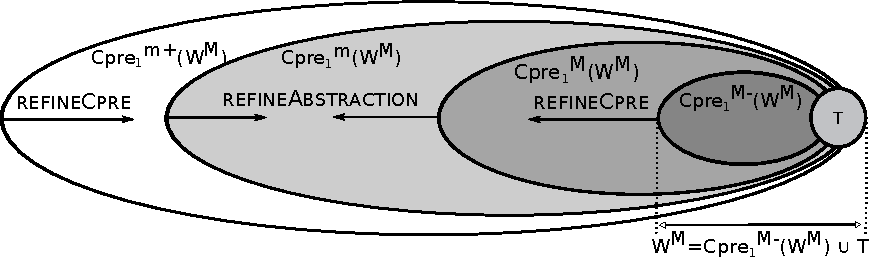
\includegraphics[width=0.85\linewidth]{imgs/approxThreeValue.pdf}
\caption{Overview of approximate three valued abstraction-refinement}
\label{fig:approx_three_val_overview}
\end{figure}


\begin{equation}
\label{eqn:cpre_p1}
\cprem \subseteq \cpremp
\end{equation}

\noindent and

\begin{equation}
\label{eqn:cpre_p2}
\cpreMm \subseteq \cpreM
\end{equation}

With these operators we create a new approximate abstraction-refinement scheme given in Algorithm \ref{alg:approx_three_val}. A graphical overview of the algorithm is given in Figure \ref{fig:approx_three_val_overview}.

\begin{algorithm}
\caption{Approximate three-valued abstraction-refinement}
\label{alg:approx_three_val}

\begin{algorithmic}[1]

\Require {\bf Input:} A game structure $G = \langle S, L, I, \tau_1, \tau_2, \delta \rangle$, a set 
of target states $T\subseteq S$, and an initial abstraction $\alpha=\langle V, \concrete{}, Cpre_1^{m+}, Cpre_1^{M-} \rangle$
that is precise for $T$, $I$, and $\tau_i$.

\Ensure {\bf Output:} {\it Yes} if $I \subseteq \reach(T, Cpre_1)$, and {\it No} otherwise.

\Function{Solve}{$transitionRelation$, $goal$}
    \Loop
        \State $W^M \gets \reach(\abstractM{T}, Cpre_1^{M-})$
        \State $W^m \gets \reach(\abstractm{T}, Cpre_1^{m+})$
        \If{$\abstractM{I} \subseteq W^M$} \Return Yes \label{alg:atv:t1}
        \ElsIf{$\abstractM{I} \nsubseteq W^m$} \Return No \label{alg:atv:t2}
        \Else       
            \State $refined \gets \Call{refineCpre}{W^M}$
            \State \algorithmicif{} {$(\neg refined)$}
                $\Call{refineAbstraction}{W^M}$
            \algorithmicend \algorithmicif
        \EndIf
    \EndLoop
\EndFunction

\end{algorithmic}
\end{algorithm}

If the algorithm terminates then it returns the correct answer. By equations \ref{eqn:cpre_p1} and \ref{eqn:cpre_p2}, 

\begin{equation}
    \reach(\abstractM{T}, \cpreMm) \subseteq \reach(\abstractM{T}, \cpreM)
\end{equation}

\noindent and 

\begin{equation}
    \reach(\abstractm{T}, \cprem) \subseteq \reach(\abstractm{T}, \cpremp)
\end{equation}

\noindent thus, by Equation \ref{eqn:cpre_inclusion}:

\begin{multline}
    \concrete{W^M} = \concrete{\reach(\abstractM{T}, \cpreMm)} \subseteq \\ \reach(T, \cpre) \subseteq \concrete{\reach(\abstractm{T}, \cpremp)} = \concrete{W^m}
\end{multline}

Thus, if we terminate on lines \ref{alg:atv:t1} or \ref{alg:atv:t2} then we terminate with the right answer.

\subsection{Initial Abstraction}

We obtain the initial abstraction by extracting atomic predicates from expressions $T$, $I$, and $\tau_i$, which guarantees that the abstraction is precise for $T$, $I$, and $\tau_i$. While this property is not essential for our approach, we will rely on it to simplify the presentation of the algorithm.

%\subsection{Initial abstraction}
%
%Algorithm~\ref{alg:generic} takes initial abstraction $\alpha$ as 
%one of its inputs. This requires fixing sets of predicates 
%$\Sigma$, $\Omega$, and $\Lambda$, and consistency relations 
%$C^{m+}$ and $C^{M-}$.  We obtain initial state predicates 
%$\Sigma$ by extracting atomic predicates from expressions $T$, 
%$I$, and $\tau_i$, which guarantees that the initial abstraction 
%is precise for $T$, $I$, and $\tau_i$, as required by the 
%algorithm.  Next, we apply the \textsc{Delta} function 
%(Algorithm~\ref{alg:delta}) to predicates in $\Sigma$ to compute 
%initial untracked and label predicates, and the abstract 
%transition relation $\Delta$.  Finally, we assign $C^{m+}=\top$ 
%and $C^{M-}=\bot$.

\subsection{Abstract controllable predecessors}
\label{s:cpre}

Following the three-valued algorithm presented in Section~\ref{sec:three_val_abs_ref}, we would like to find an efficient way to compute over- and under-approximations $Cpre^{m+}$ and $Cpre^{M-}$ of the abstract controllable predecessor operators. Recall that computing $Cpre^m$ and $Cpre^M$ precisely is expensive, as it requires applying the controllable predecessor operator to the concrete transition relation $\delta$. We approximate this costly computation by computing the controllable predecessor over the \emph{abstract transition relation} instead. The abstract transition relation of the game is defined over boolean predicate variables and therefore can be manipulated much more efficiently than the concrete one.

We construct the abstract transition relation via efficient syntactic analysis of the concrete transition relation $\delta$. We present the construction assuming that $\delta$ is given in the variable update form, as in Figure~\ref{f:ex}c. A similar construction is possible for specifications written in real-world hardware and software description languages.

For each state predicate in $\Sigma$, we compute the update function by replacing concrete variables in the predicate with their corresponding update functions. We then transform the resulting formula into a boolean combination of atomic predicates over concrete state and label variables.

\begin{ex}
    Let us compute the update function for abstract variable $\sigma_1$ (Figure~\ref{f:ex}d).  Using update functions for $req$ and $dat$ variables (Figure~\ref{f:ex}c), we obtain: 
    
    \begin{multline}
    \sigma_1' = (req' = dat') = \neg(bsy = false) \land (req=dat) \\ \lor (bsy=false) \land (val=req)
    \end{multline}
    
    \noindent This equation contains three atomic predicates: in addition to the existing predicate $\sigma_1 \leftrightarrow (req=dat)$, it introduces new predicates $(bsy=false)$ and $(val=req)$.  

    The first two predicates correspond to existing state variables $\sigma_1$ and $\sigma_2$.  The last predicate is new; hence it is added to set $\Omega$ and a new untracked variable $\omega_1$ is created for it.  By substituting predicates in the equation with corresponding abstract variables, we obtain the following abstract transition relation for $\sigma_1$ in line~11 of the algorithm:
    $\sigma_1' = (\overline{\sigma_2} \land \omega_1) \lor (\sigma_2 \land \sigma1)$
    \qed
\end{ex}

In the general case, the syntactically computed update function for a predicate may depend on existing state predicates in $\Sigma$ as well as new predicates that are not yet part of the abstraction.  The new predicates are partitioned into \emph{untracked predicates} defined over concrete state variables (e.g., $\mathtt{bsy=false}$ in the above example) and \emph{label predicates} that involve at least one concrete label variable (e.g., $\mathtt{val=req}$).  The term ``untracked predicate'' indicates that these predicates are not part of the abstract state space of the game.  Untracked predicates can be seen as partitioning abstract states in $V$ into smaller \emph{untracked sub-states}, as illustrated in Figure~\ref{f:predicates}.

By substituting untracked and label predicates with fresh boolean variables, $\vect{\omega}$ and $\vect{\lambda}$ respectively, we obtain the abstract transition relation $\Delta$ in the form:

$$
\vect{\sigma}'=\Delta(\vect{\sigma},\vect{\omega},\vect{\lambda})
$$

This syntactically computed transition relation contains two sources of imprecision.  First, untracked variables $\vect{\omega}$ are not part of the abstract state space $\Sigma$ and are therefore treated as external inputs.  Second, not all abstract labels  are available in all abstract states and hence not all transitions in $\Delta$ correspond to a feasible concrete transition.  For example, given the set of predicates shown in Figure~\ref{f:ex}d, the abstract label $\lambda_1 = true, \lambda_2 = true$ is only available in concrete states that satisfy the condition $req=5$.  In general, given a state-untracked-label tuple $\langle v,u,l\rangle$, the abstract label $l$ may be available in all, some, or none of the concrete states consistent with $v$ and $u$.  

We formalise this by introducing \emph{consistency relations} $C^m$ and $C^M$ that over- and under-approximate available abstract labels.  A state-untracked-label tuple $\langle v,u,l\rangle$ is \emph{may-consistent} if the abstract label $l$ is available in \emph{at least one} concrete state consistent with $v$ and $u$:

\begin{equation} \label{e:Cm}
    C^m(v,u,l) = \exists X,Y. \|\vect{\sigma}\|=v \land \|\vect{\omega}\|=u \land \|\vect{\lambda}\|=l.
\end{equation}

The tuple $\langle v,u,l\rangle$ is \emph{must-consistent} if $l$ is available in \emph{any} concrete state consistent with $v$ and $u$:

\begin{equation}
    C^M(v,u,l) = \forall X . ((\|\vect{\sigma}\|=v \land \|\vect{\omega}\|=u) \rightarrow \exists Y.  \|\vect{\lambda}\|=l)
\end{equation}

Computing $C^m$ and $C^M$ can be prohibitively expensive.  Therefore we use approximations $C^{m+}$ and $C^{M-}$ such that $C^m\subseteq C^{m+}$ and $C^{M-}\subseteq C^M$.  Initially we assign $C^{m+}=\top$ and $C^{M-}=\bot$.  Approximations are refined lazily as part of the abstraction refinement process, as explained below.

\begin{ex}
    \everymath{\mathtt{\xdef\tmp{\fam\the\fam\relax}\aftergroup\tmp}}
    \everydisplay{\mathtt{\xdef\tmp{\fam\the\fam\relax}\aftergroup\tmp}}
    To illustrate the above definitions, we introduce two label predicates to our running example: $\|\lambda_1\|= (val=req)$, $\|\lambda_2\| = (val=5)$. Consider the state-untracked-label tuple $v=(true,false)$, $u=(true)$, $l=(true, true)$, which corresponds to the following assignment to abstract variables: $\sigma_1=true \land \sigma_2=false \land \omega_1=true \land \lambda_1=true \land\lambda_2=true$. It is easy to see that this condition is satisfied for example by the following concrete variable valuation: $mem=5$, $dat=5$, $bsy=true$, $req=5$, $val=5$, hence $\langle v,u,l\rangle$ is may-consistent: $C^m(v,u,l)=true$.  However, it is not must-consistent:

    $$
    \begin{aligned}
        C^M(v,u,l) = \forall  mem, dat, bsy,req. (&((req=mem) \land (bsy = true) \land (req=dat)) \rightarrow \\
                                                  &\exists val. (val=req) \land (val=5))
    \end{aligned}
    $$
    
    There exist concrete state variable assignments (e.g., $mem=1$, $dat=1$, $bsy=true$, $req=1$) that satisfy state and untracked predicates in the left-hand side of the implication but that can not be extended with a label variable assignment that satisfies the right-hand side, hence $C^M(v,u,l)=false$.  
    \qed
\end{ex}

We compute over- and under-approximations of the controllable predecessor operator by resolving the two sources of imprecision in favour of one of the players.  In particular, we compute $Cpre_i^{m+}$ by (1) allowing player $i$ to pick assignments to untracked predicates, (2) over-approximating consistent labels available to $i$, and (3) under-approximating consistent labels available to the opponent player $\overline{i}$:

\begin{equation}
    \label{e:cprem}
    \small
\begin{aligned}
    Cpre_i^{m+}(\phi) = \exists \vect{\omega} .~&\abstractM{\tau_i}         \land \exists \vect{\lambda},\vect{\sigma'}. ((C^{m+} \land \Delta) \land \phi')
                                                 ~~\lor\\
                                                &\abstractM{\tau_{\overline{i}}} \land \forall \vect{\lambda},\vect{\sigma'}. ((C^{M-} \land\Delta) \rightarrow \phi')
\end{aligned}
\end{equation}

This formula has a similar structure to the definition of the concrete controllable predecessor operator (\ref{e:cpre}).  It replaces the concrete transition relation $\delta$ with the abstract transition relation $\Delta$ restricted with consistency relations ($C^{m+}$ and $C^{M-}$).  In addition, it existentially quantifies untracked variables $\vect{\omega}$, i.e., an abstract state $v$ is a may-predecessor of $\phi$ if at least one of its untracked sub-states is a may-predecessor of $\phi$.

Dually, we compute $Cpre_i^{M-}$ by (1) allowing the opponent player $\overline{i}$ to pick values of untracked predicates, (2) under-approximating labels available to $i$ and (3) over-approximating labels available to $\overline{i}$:

\begin{equation}
    \small
    \label{e:cpreM}
\begin{aligned}
    Cpre_i^{M-}(\phi) = \forall \vect{\omega}.~&\abstractM{\tau_i}         \land \exists \vect{\lambda},\vect{\sigma'}. ((C^{M-} \land \Delta) \land \phi')
                                             ~~\lor\\
                                               &\abstractM{\tau_{\overline{i}}} \land \forall \vect{\lambda},\vect{\sigma'}. ((C^{m+} \land \Delta) \rightarrow \phi')
\end{aligned}
\end{equation}

Note that the use of $C^{m+}$ and $C^{M-}$ in (\ref{e:cprem}) and (\ref{e:cpreM}) under-constrains moves available to player~$i$ and over-constrains moves available to the opponent.  The formula for $CpreU_i^{M-}(\phi)$ is analogous, except that it over-constrains moves available to $i$ and under-constrains moves available to $\overline{i}$.

Equations (\ref{e:cprem}) and (\ref{e:cpreM}) suggest two possible abstraction refinement tactics, which correspond to the two types of refinement used in Algorithm~\ref{alg:generic}.  First, we can refine $C^{m+}$ and $C^{M-}$ by removing spurious transitions from $C^{m+}$ or adding new consistent transitions to $C^{M-}$.  Such a refinement increases the precision of controllable predecessor computation without introducing new state predicates, which corresponds to the \textsc{refineCpre} operation in the algorithm.  Second, we can add some of the untracked predicates to the set of state predicates $\Sigma$, thus reducing the imprecision introduced by treating them as external inputs.  This refinement increases the precision of the abstraction, which corresponds to the \textsc{refineAbstraction} function in the algorithm.

In summary, we solve the abstract game by decomposing potentially expensive computations into three types of light-weight operations performed on demand, as required to improve the precision of the abstraction:

\begin{itemize}
    \item Computing the abstract transition relation $\Delta$ via 
        light-weight syntactic analysis of the concrete game
    \item Computing consistency relations $C^{m+}$ and $C^{M-}$ by 
        iteratively identifying spurious and consistent 
        transitions
    \item Solving the abstract game using abstract controllable 
        predecessor operators (\ref{e:cprem}) and (\ref{e:cpreM})
\end{itemize}

The computational bottleneck in this method can arise either from having to perform an excessive number of refinements or if abstractions generated by the algorithm are too complex.  Our refinement procedures, described below, are designed to avoid such situations by heuristically picking refinements that are likely tospeed up the convergence of the algorithm.

%\subsection{Abstract transition relation}
%
%The \emph{abstract transition relation}
%$\Delta: \mathbb{B}^n \times \mathbb{B}^k \times \mathbb{B}^m 
%\rightarrow 2^{\mathbb{B}^n}$
%of the game maps an assignment of state, untracked, and label 
%predicates to the set of possible next states.  The arrow in 
%Figure~\ref{f:predicates} illustrates a transition from untracked 
%sub-state $u$ of state $v$ to state $v'$ via abstract label $l$.  
%Note that the source of an abstract transition is a pair of state 
%and untracked predicate assignments, while the target of the 
%transition is an assignment to state predicates only.
%
%Algorithm~\ref{alg:delta} shows the pseudocode of function 
%\textsc{Delta}.  It takes a list of state predicates and returns 
%the abstract transition relation $\Delta$ along with untracked and 
%label predicates used in $\Delta$.
%It assumes that the concrete transition relation $\delta$ of the 
%game is specified in the form of variable update functions $x' = 
%t_x(X,Y)$, as in Figure~\ref{f:ex}b.
%
%\begin{algorithm}[t]
%\caption{Pseudocode for computing the abstract transition relation.}
%\label{alg:delta}
%\begin{algorithmic}[1]
%    \Function{Delta}{$\vect{\sigma}=(\sigma_1\ldots\sigma_n)$ - state predicate variables}
%        \For{$i = 1 \text{ to } n$}
%            \State $t_{\sigma_i} \gets \|\sigma_i \|[x \mid t_x(X,Y), \text{for all } x\in X]$
%            \State $t_{\sigma_i} \gets $ \Call{massage}{$t_{\sigma_i}$}
%        \EndFor
%        \State $P \gets \bigcup_i \text{atomic predicates in }t_{\sigma_i}$
%        \State $\Omega \gets \text{state predicates in } P \setminus \Sigma$
%        \State $\Lambda \gets \text{label predicates in } P \setminus \Sigma$
%        \State $\vect{\omega}\gets \text{fresh variables for predicates in } \Omega$
%        \State $\vect{\lambda} \gets \text{fresh variables for predicates in } \Lambda$
%        \State $\Delta \gets \bigwedge_i (\sigma_i' = t_{\sigma_i}[\|\alpha\|\mid \alpha, \text{for all } \alpha\in\vect{\sigma}\cup\vect{\omega}\cup\vect{\lambda}])$
%        \State \Return $\langle \vect{\omega}, \vect{\lambda}, \Delta \rangle$
%    \EndFunction
%\end{algorithmic}
%\end{algorithm}
%
%Lines 2--5 of the algorithm compute update functions for predicate 
%variables $\sigma_i$ by replacing each variable $x$ in predicate 
%$\|\sigma_i\|$ by its update function $t_x$.  The \textsc{massage} 
%function transforms the resulting expression $t_{\sigma_i}$ into a 
%boolean combination of atomic predicates over $X \cup Y$.  In 
%line~6 we collect all predicates found in $t_{\sigma_i}$.  The 
%resulting set $P$ may contain predicates not found in $\Sigma$.  
%Such predicates are classified into untracked predicates $\Omega$ 
%defined over state variables only and label predicates $\Lambda$ 
%that involve at least one label variable from $Y$ (lines~7--8).  
%The abstract transition relation $\Delta$ is computed by replacing 
%all boolean predicates in $t_{\sigma_i}$ with corresponding 
%boolean variables (line~11).
%
%\begin{ex}
%    \everymath{\mathtt{\xdef\tmp{\fam\the\fam\relax}\aftergroup\tmp}}
%    \everydisplay{\mathtt{\xdef\tmp{\fam\the\fam\relax}\aftergroup\tmp}}
%    Let us compute the update function for abstract variable 
%    $\sigma_1$. Recall that $\|\sigma_1\| = (req=mem)$.  Using 
%    update functions for $req$ and $mem$ variables from 
%    Figure~\ref{f:ex}b, we obtain:
%    $t_{\sigma_1} = (t_{req}(X,Y)=t_{mem}(X,Y)) = \bigg(req = 
%    \begin{cases}
%        dat, & \text{if } \neg bsy\\
%        mem, & \text{otherwise}
%    \end{cases}\bigg).$  The \textsc{massage} function transforms 
%    this into:
%    $t_{\sigma_1} = \big((bsy = true \land req=dat) \lor 
%    (bsy=false \land req=mem)\big)$.
%    This equation contains three predicates: $(req=mem)$, 
%    $(bsy=false)$ (and its negation), and $(req=dat)$.  The first 
%    two predicates correspond to existing state variables 
%    $\sigma_1$ and $\sigma_2$.  The last predicate is new; hence 
%    it is added to set $\Omega$ and a new untracked variable 
%    $\omega_1$ is created for it.  By substituting predicates in 
%    the equation with corresponding abstract variables, we obtain 
%    the following abstract transition relation for $\sigma_1$ in 
%    line~11 of the
%    algorithm:
%    $\sigma_1' = (\overline{\sigma_2} \land \omega_1) \lor (\sigma_2 \land \sigma1)$
%    \qed
%\end{ex}
%
%The above algorithm has the useful property that $\Delta$ is 
%computed via simple syntactic transformations of the concrete 
%game specification. Additionally, untracked predicates discovered 
%by the algorithm are known to influence the values of state 
%predicates in $\Sigma$. As such, these predicates constitute 
%potentially useful candidates for promotion to state predicates 
%as part of the abstraction refinement process.

\begin{algorithm}
\caption{Three-valued abstraction refinement for games.}
\label{alg:genericc}

\begin{algorithmic}[1]

\Function{Solve}{$transitionRelation$, $goal$}
    \Statex {\bf Input:} A game structure $G = \langle S, L, I, \tau_1, \tau_2, \delta \rangle$, a set 
    of target states $T\subseteq S$, and an initial abstraction $\alpha=\langle V, \concrete{}, Cpre_1^{m+}, Cpre_1^{M-} \rangle$
    that is precise for $T$, $I$, and $\tau_i$.

    \Statex {\bf Output:} {\it Yes} if $I \subseteq \reach(T, Cpre_1)$, and {\it No} otherwise.

    \Loop
        \State $W^M \gets \reach(\abstractM{T}, Cpre_1^{M-})$
        \State $W^m \gets \reach(\abstractm{T}, Cpre_1^{m+})$
        \If{$\abstractM{I} \subseteq W^M$} 
            \State\Return Yes
        \ElsIf{$\abstractM{I} \nsubseteq W^m$} 
            \State\Return No
        \Else       
            \State $refined \gets \Call{refineCpre}{W^M}$
            \If {$(\neg refined)$}
                \State$\Call{refineAbstraction}{W^M}$
            \EndIf
        \EndIf
    \EndLoop
\EndFunction

\end{algorithmic}
\end{algorithm}

\subsection{Consistency Refinement}

Figure~\ref{f:crefinement} illustrates the main idea of the consistency refinement algorithm.  It shows an abstract state $v$ (Figure~\ref{f:crefinement}a) at the may-must boundary whose untracked substates $u_1$, $u_2$, and $u_3$ have $C^{m+}$-consistent transitions to the must-winning set $W^M$, but none of these transitions is consistent with $C^{M-}$.  The \textsc{refineCpre} algorithm attempts to precisely categorise these substates as must-winning or must-losing.

Since all untracked substates of $v$ are either must-losing or may-winning but not must-winning, it is impossible to split out a must-winning subset of $v$ purely by predicate promotion; hence a consistency refinement is needed.

The consistency refinement algorithm proceeds in one of three ways:
\begin{itemize}
    \item In Figure~\ref{f:crefinement}b, the algorithm identifies the abstract transition $\langle v,u_1, l_1\rangle$ as spurious and eliminates it from $C^{m+}$, thus making the $u_1$ sub-state must-losing.  
    \item Alternatively, it may detect that abstract transition $\langle v, u_2, l_2\rangle$ is available in all concrete states in $u_2$ and thus add this transition to $C^{M-}$, making the $u_2$ sub-state must-winning (Figure~\ref{f:crefinement}c).  
    \item Finally, it may determine that abstract transition $\langle v, u_3, l_3\rangle$ is available in some, but not all, concrete states in $u_3$, i.e., $\langle v, u_3, l_3\rangle\in C^m\setminus C^M$.  It then partitions $u_3$ into two or more subsets, exactly one of which has a $C^{M-}$-consistent transition to $W^M$, by introducing new untracked predicates (Figure~\ref{f:crefinement}d).  
\end{itemize}

In all three cases, further refinement via untracked predicate promotion becomes possible.  Such refinement is performed by the \textsc{refineAbstraction} function described in Section~\ref{s:refineAbstraction}.

\begin{figure}[t]
    \label{f:crefinement}
    \center
    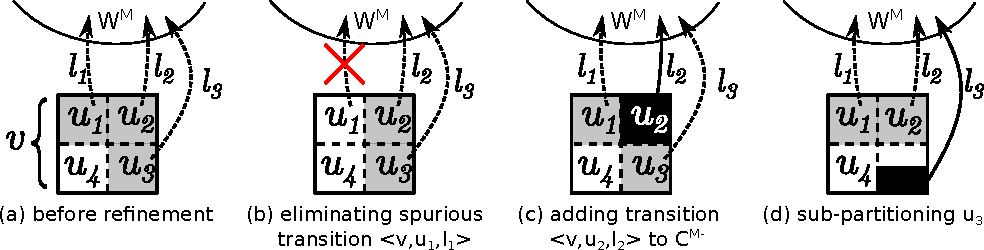
\includegraphics[width=\linewidth]{imgs/crefinement}
    \caption{Different types of consistency refinements.  White, grey, and black background is used to mark respectively must-losing, may-winning, and must-winning untracked substates.  Dashed and solid arrows show $C^{m+}$ and $C^{M-}$-consistent abstract transitions.}
\end{figure}

Note that in the special case when, after performing consistency refinement, all untracked substates of $v$ become must-winning or must-losing, the entire state $v$ can be removed from the boundary region without performing predicate promotion.  This corresponds to the two types of refinement labelled as \textsc{refineCpre} in Figure~\ref{f:reach}.  

For this reason, Algorithm~\ref{alg:generic} recomputes $W^M$ and $W^m$ after each successful consistency refinement, and only calls \textsc{refineAbstraction} once no more consistency refinements are possible.

\subsubsection{Algorithm}

Algorithm~\ref{alg:refineCpre} shows the pseudocode of \textsc{refineCpre}.  Lines~3--6 compute the set of candidate tuples $\langle v, u, l\rangle\in C^m\setminus C^M$.  Note that for player~$i$ states we consider may-consistent transition to $W^M$, whereas for player~$\overline{i}$ states we consider spoiling transitions to $V\setminus W^M$.

Line~9 picks a single refinement candidate $\langle v,u,l \rangle$ from the set.  By construction we know that $\langle v,u,l\rangle\in C^{m+}$.  Since $C^{m+}$ is an overapproximation of $C^m$, we check whether $\langle v,u,l\rangle\in C^m$, i.e., whether $v$, $u$, and $l$ satisfy equation (\ref{e:Cm}).  To this end, in line~11 we invoke a decision procedure for the underlying theory to check satisfiability of the formula:$(\|\vect{\sigma}\|=v \land \|\vect{\omega}\|=u \land \|\vect{\lambda}\|=l)$.If the formula is unsatisfiable, then $\langle v,u,l\rangle$ is a spurious transition that must be eliminated from $C^{m+}$.  Furthermore, by extracting an unsatisfiable core of the formula,we obtain an inconsistent subset of its conjuncts $(\bigwedge\|\alpha_i\|=c_i)$, $\alpha_i\in\vect{\sigma}\cup\vect{\omega}\cup\vect{\lambda}$,which represents a potentially large set of similar spurioustransitions.  We eliminate all of these transitions from $C^{m+}$ inline~16.

\begin{algorithm}[t]

\caption{Pseudocode of the \textsc{refineCpre} function}
\label{alg:refineCpre}
\begin{algorithmic}[1]
\Function{refineCpre}{$W^M$}
    \State \Comment{player~$i$ may-winning transitions}
    \State $T_i         \gets \abstractM{\tau_i} \land C^{m+} 
    \land {\overline{C^{M-}}} \land \forall \vect{\sigma'}. (\Delta \rightarrow (W^M)')$
    \State \Comment{player~$\overline{i}$ may-spoiling transitions}
    \State $T_{\overline{i}} \gets \abstractM{\tau_{\overline{i}}} \land C^{m+} \land {\overline{C^{M-}}} \land \exists \vect{\sigma'}. (\Delta \land \overline{(W^M)'})$
    \State $T           \gets T_i \lor T_{\overline{i}}$
    \If{$T = \bot$}
        \Return $false$ \Comment{no refinement is possible}
    \Else
        \State choose $\langle v,u,l\rangle \in T$
        \State $F \gets (\|\vect{\sigma}\|=v \land \|\vect{\omega}\|=u \land \|\vect{\lambda}\|=l)$
        \If{\Call{satisfiable}{$F$}}
            \State $A             \gets $ \Call{eliminateQuantifiers}{$\exists Y.\|\vect{\lambda}\|=l$}
            \State $A             \gets $ \Call{massage}{$A$}
            \State $P             \gets \text{atomic predicates in }A$
            \State $\vect{\omega} \gets \vect{\omega} \cup (\text{fresh variables for predicates in } P\setminus\Omega)$
            \State $\Omega        \gets \Omega \cup P$
            \State $\hat{A}       \gets A[\|x\|\mid x, \text{for all } x\in\Omega \cup \Sigma ]$
            \State $\hat{A}       \gets$ replace atomic predicates in $A$ with boolean
            \Statex  ~~~~~~~~~~~~~~~~~~~~vars, introducing fresh vars when necessary
            \State $C^{M-}        \gets C^{M-} \lor (\hat{A}\land \vect{\lambda}=l)$% \Comment{add consistent transition}
        \Else
%            \State $(\bigwedge\|\alpha_i\|=c_i) \gets$ \Call{unsatCore}{$F$}
            \State $C^{m+}\gets C^{m+} \land \overline{\textsc{unsatCore}(F)}$ %\Comment{eliminate spurious transitions}
        \EndIf
        \State \Return $true$
    \EndIf
\EndFunction
\end{algorithmic}
\end{algorithm}

If, on the other hand, the formula is satisfiable, then there exists a concrete state-label pair consistent with $\langle v,u,l\rangle$.  In this case we want to precisely characterise the set of states where label $l$ is available, so that we can either add $\langle v,u,l\rangle$ to $C^{M-}$ (as in Figure~\ref{f:crefinement}c) or refine it with additional untracked predicates (as in Figure~\ref{f:crefinement}d).

Line~12 computes the set of concrete states where abstract label $l$ is available by performing quantifier elimination from formula $(\exists Y.\|\vect{\lambda}\|=l)$, resulting in a quantifier-free formula $A$ over concrete state variables $X$.  We assume that the underlying theory supports quantifier elimination, which is the case for many practically relevant theories, including the theory of fixed-size bit vectors supported by our tool.  In line~13, the resulting formula $A$ is decomposed into atomic predicates possibly introducing new untracked and label predicates.  By replacing all atomic predicates in $A$ with corresponding boolean variables, we obtain a formula $\hat{A}$ that describes the set of all state-untracked pairs must-consistent with the abstract label $l$.  Line~14 refines $C^{M-}$ with the set of newly discovered must-consistent transitions.

%The resulting formula is decomposed into atomic predicates 
%(lines~11--12).  New predicates from $A$ are added to the set of 
%untracked predicates (lines~13--14).  Finally, all predicates in 
%$A$ are replaced with corresponding boolean variables (line~15) 
%and the resulting formula over abstract variables is used to 
%refine the must consistency relation $C^{M-}$ (line~16).  

\begin{ex}
    \everymath{\mathtt{\xdef\tmp{\fam\the\fam\relax}\aftergroup\tmp}}
    \everydisplay{\mathtt{\xdef\tmp{\fam\the\fam\relax}\aftergroup\tmp}}
    Assume that in line~9 the algorithm picks a tuple $\langle 
    v,u,l\rangle$ where $l=(true, true)$.  Line~12 performs 
    quantifier elimination from the formula $\exists val.  
    (\|\lambda_1\|=true \land  \|\lambda_2\|=true) =
    \exists val. (val=req \land val=5) = (req=5)$.
%    , i.e., conditions $(val=req)$ and $(val=5)$ can only hold 
%    simultaneously if $(req=5)$.
    We have discovered a new predicate $req=5$ that 
    must hold in states where abstract label $l$ is 
    available.  We introduce a new untracked variable $\omega_2$, 
    $\|\omega_2\|=(req=5)$ and refine $C^{M-}$ with a new 
    consistent transition: $C^{M-} \gets C^{M-} \lor (\omega_2 
    \land \lambda_1 \land \lambda_2)$.
    \qed
\end{ex}

\subsection{Refining the Abstraction}
\label{s:refineAbstraction}

The \textsc{refineAbstraction} function is invoked by the abstraction refinement algorithm when no further consistency refinements are possible.  At this point, every untracked sub-state of the boundary region is either must-winning or must-losing, i.e., can be coloured white or black using notation of Figure~\ref{f:crefinement}.  \textsc{refineAbstraction} promotes a subset of untracked predicates making sure that the winning region $W^M$ expands after re-solving the game in line~2 of Algorithm~\ref{alg:generic}.  

Algorithm~\ref{alg:refineAbstraction} shows the pseudocode of \textsc{refineAbstraction}.  Line~2 computes all untracked boundary substates that are must-predecessors of $W^M$.  Here, $CpreU^{M-}$ is the same as $Cpre^{M-}$ (Equation~(\ref{e:cpreM})), but without untracked variable quantification:

$$
    \small
\begin{aligned}
    CpreU_i^{M-}(\phi) = &\abstractM{\tau_i}         \land \exists \vect{\lambda},\vect{\sigma'}. ((C^{M-} \land \Delta) \land \phi')
                          ~~\lor\\
                         &\abstractM{\tau_{\overline{i}}} \land \forall \vect{\lambda},\vect{\sigma'}. ((C^{m+} \land \Delta) \rightarrow \phi')
\end{aligned}
$$

We aim to grow  $W^M$ by promoting as few untracked predicates as possible.  To this end, we extract a short prime implicant from $U^M$ and promote the untracked variables in the support of the prime implicant(line~3).  This has the effect of adding a large cube over state and untracked predicates to $W^M$. The \textsc{promote} function invoked in line~4 moves the selected untracked predicates to the set of state predicates $\Sigma$ and recomputes the abstraction transition relation $\Delta$ for the new state predicates.  This can lead to the introduction of new untracked and label predicates, which can serve as refinement candidates in the future.

\begin{algorithm}[t]

\caption{Pseudocode of \textsc{refineAbstraction}}
\label{alg:refineAbstraction}

\begin{algorithmic}[1]

\Function{refineAbstraction}{$W^M$}
    \State $U^M \gets CpreU_1^{M-}(W^M) \land \overline{W^M}$
    \State $toPromote \gets \vect{\omega}~\cap~$\Call{support}{\textsc{shortPrime}($U^M$)}
    \State $\Call{promote}{toPromote}$
\EndFunction

\end{algorithmic}
\end{algorithm}

\subsection{Enabling Variables}

Algorithm~\ref{alg:refineCpre} has an important performance issue: 
in lines~10--16 it analyses and adds to $C^{M-}$ a single abstract 
label $l$.  The set of all abstract labels is exponential in size 
in the number of label predicates and can be very large in 
practice, making explicit enumeration infeasible.  We therefore 
modify the algorithm to handle a set of abstract labels at every 
iteration.  To this end, in line~7, instead of choosing a complete 
assignment to state, untracked, and label predicates, we compute a 
\emph{prime implicant} of set $T$, i.e., an assignment to a subset 
of variables in $\vect{\sigma}\cup\vect{\omega}\cup\vect{\lambda}$ 
such that any extension of this assignment to the remaining 
variables satisfies $T$:
$$\langle v,u,l\rangle \gets \textsc{primeImplicant}(T),$$
where $v$, $u$, and $l$ are partial valuations of abstract 
variables, which compactly represent a potentially large set of 
abstract transitions.  In practice, we typically discover prime 
implicants that only constrain few of the abstract variables, 
meaning that other predicates are irrelevant for the outcome of 
the transition.  

%Next, we modify lines~9 and 14 to 


Given this modification, the $C^{m+}$ refinement case of the 
algorithm (lines~18--19) is still correct and does not require any 
changes.  However, changes are needed in the $C^{M-}$ refinement 
logic.  The set $A$ computed in lines~10--1 contains all
concrete states where \emph{at least one} abstract label from the 
set characterised by the partial assignment $l$ of label 
predicates is available.  It does not guarantee the availability 
of any particular label from this set.  To model this constraint, we would have 
to change $C^{M-}$ to be a relation over sets of labels.  Every 
element of the relation would describe a set of labels, one of 
which is guaranteed to be available for the given state and 
untracked predicate assignment.  

This introduces a new form of imprecision to the consistency 
relation: rather than categorising each abstract label as 
available or unavailable in the given state, we record a set of 
labels, one of which is available.  However, such a relation would 
be hard to represent and manipulate efficiently in the symbolic 
form.  Therefore, we propose a different approach that allows 
symbolic implementation.  

We transform the game (without changing its winning set) in order 
to solve it more efficiently.  The idea of our solution is to 
model the new form of imprecision as non-determinism in the 
abstract transition relation $\Delta$.  For each abstract label 
variable $\lambda_i$, we introduce an auxiliary \emph{enabling 
variable} $\varepsilon_i$ and transform the transition relation 
$\Delta$ as follows:
$$\Delta \gets (\varepsilon_i \land \Delta) \lor (\overline{\varepsilon_i} \land \exists \lambda_i. \Delta).$$
When $\varepsilon_i=true$, $\Delta$ behaves exactly as before.  In 
case $\varepsilon_i=false$, the value of $\lambda_i$ chosen by the 
player is ignored and the environment non-deterministically 
selects next-state variables assignment that is consistent with 
\emph{some} assignment of $\lambda_i$. 

We can now modify line~16 of Algorithm~\ref{alg:refineCpre} as 
follows:
$$
C^{M-} \gets C^{M-} \lor (\hat{A}\land \bigwedge_{i\in{j_1\ldots j_p}}\lambda_i=l_i \land \bigwedge_{i\not\in{j_1\ldots j_p}}\varepsilon_i=false),
$$
where $j_1\ldots j_p$ are indices of variables assigned by $l$.  
The above statement refines $C^{M-}$ by allowing the player to 
assign a subset of label variables in accordance with $l$ and
disabling other label variables not constrained by $l$.  The 
environment will non-deterministically pick arbitrary values for 
these variables.  In this way we precisely capture what we 
currently know about consistent predicate assignments in a
a symbolic form, at the cost of introducing extra variables 
$\varepsilon_i$.
